%\pdfoutput=1
\documentclass[12pt,a4paper,reqno]{amsart}
\newcommand\hmmax{0}
\newcommand\bmmax{0}
\usepackage{amssymb}
\usepackage{amscd}
\usepackage[pdftex,pdfpagelabels]{hyperref}
\usepackage{enumerate}
\usepackage{comment}
%\usepackage{psfig}
\usepackage{graphicx}
\usepackage{cleveref}
\usepackage{siunitx}
\usepackage{tikz-cd}
\usepackage{stix}
\usepackage{bm}
\DeclareMathAlphabet\mathbfcal{LS2}{stixcal}{b}{n}
\numberwithin{equation}{section}

%\usepackage{mathabx}


\usepackage{mathtools}%                  http://www.ctan.org/pkg/mathtools
\usepackage[tableposition=top]{caption}% http://www.ctan.org/pkg/caption
\usepackage{booktabs,dcolumn}%           http://www.ctan.org/pkg/dcolumn + http://www.ctan.org/pkg/booktabs

% Lighter notation.
%\newcommand*\mc[1]{\multicolumn{1}{c}{#1}}
%\newcommand*\tupref[2]{\href{http://math.mit.edu/~primegaps/tuples/admissible_#1_#2.txt}{\num{#2}}}



%\DeclareMathOperator*\Kl{Kl} (commented because yield bad display for  \Kl_q %replaced with \newcommand... )
%\DeclareMathOperator*\FT{FT} (commented because yield bad display for \FT_q
%replaced with \newcommand...)

\DeclareMathOperator*\swan{swan}
\DeclareMathOperator*\cond{cond}
\DeclareMathOperator*\Gal{Gal}

\newcommand{\FT}{\mathrm{FT}}
\newcommand{\Kl}{\mathcal{K}\ell}
% Setup for ``caption''.
%\DeclareCaptionLabelSeparator{separation}{:\quad}
%\captionsetup{
  %font=small,
  %labelfont=sc,
  %labelsep=separation,
  %width=0.8\textwidth
%}

\DeclareFontFamily{OT1}{rsfs}{}
\DeclareFontShape{OT1}{rsfs}{n}{it}{<-> rsfs10}{}
\DeclareMathAlphabet{\mathscr}{OT1}{rsfs}{n}{it}

\addtolength{\textwidth}{3 truecm}
\addtolength{\textheight}{1 truecm}
\setlength{\voffset}{-.6 truecm}
\setlength{\hoffset}{-1.3 truecm}

\theoremstyle{plain}

\newtheorem{theorem}{Theorem}[section]
%\newtheorem{theorem}[theorem]{Theorem}
\newtheorem{proposition}[theorem]{Proposition}
\newtheorem{lemma}[theorem]{Lemma}
\newtheorem{corollary}[theorem]{Corollary}
\newtheorem{conjecture}[theorem]{Conjecture}
\newtheorem{heuristic}[theorem]{Heuristic}
\newtheorem{principle}[theorem]{Principle}
\newtheorem{question}[theorem]{Question}
\newtheorem{problem}[theorem]{Problem}
\newtheorem{claim}[theorem]{Claim}

\theoremstyle{definition}

%\newtheorem{roughdef}[subsection]{Rough Definition}
\newtheorem{definition}[theorem]{Definition}
\newtheorem{remark}[theorem]{Remark}
\newtheorem{remarks}[theorem]{Remarks}
\newtheorem{example}[theorem]{Example}
\newtheorem{examples}[theorem]{Examples}
%\newtheorem{problem}[subsection]{Problem}
%\newtheorem{question}[subsection]{Question}

\renewcommand\P{\mathbb{P}}
\newcommand\E{\mathbb{E}}
\newcommand\Var{\mathrm{Var}}
\newcommand\R{\mathbb{R}}
\newcommand\Z{\mathbb{Z}}
\newcommand\F{\mathbf{F}}
\newcommand\N{\mathbb{N}}
\newcommand\n{\mathbf{n}}
\renewcommand\a{\mathbf{a}}
\renewcommand\b{\mathbf{b}}
\renewcommand\j{\mathbf{j}}
\renewcommand\k{\mathbf{k}}
\renewcommand\v{\mathbf{v}}
\renewcommand\t{\mathbf{t}}
\renewcommand\r{\mathbf{r}}
\renewcommand\l{\mathbf{l}}
\newcommand\X{\mathbf{X}}
\newcommand\T{\mathbf{T}}
\newcommand\Y{\mathbf{Y}}
\newcommand\A{\mathbf{A}}
\newcommand\W{\mathbf{W}}
\newcommand\C{\mathbb{C}}
\newcommand\Q{\mathbb{Q}}
\renewcommand\Re{{\operatorname{Re}}}
\renewcommand\Im{{\operatorname{Im}}}
\newcommand\Log{{\operatorname{Log}}}
\newcommand\lcm{{\operatorname{lcm}}}
\renewcommand\gcd{{\operatorname{gcd}}}
\newcommand\eps{\varepsilon}
\newcommand\tuple{{\mathcal B}}
\newcommand\excess{{\mathrm{E}}}

\renewcommand{\mod}{\bmod}

\parindent 0mm
\parskip   5mm


\begin{document}

\title{Notes on upper and lower bounding $t(N)$}

\author{Terence Tao}
\maketitle

%%%%%%%%%%%%%%%%%%%%%%%%%%%%%%%%%%%%%%%%%%%%%%%%%

\section{Basics}

The symbol $p$ will always denote a prime.  The primes $2,3$ will play a special role here and will be referred to as \emph{tiny primes}.

We use $\nu_p(a/b) = \nu_p(a)-\nu_p(b)$ to denote the $p$-adic valuation of a positive natural number $a/b$, that is to say the number of times $p$ divides the numerator $a$, minus the number of times $p$ divides the denominator $b$.  For instance, $\nu_2(32/27)=5$ and $\nu_3(32/27)=-3$. 
If one applies a logarithm to the fundamental theorem of arithmetic, one obtains the identity
\begin{equation}\label{ftoa}
  \sum_p \nu_p(r) \log p = \log r
\end{equation}
for any positive rational $r$.

Asymptotically, it is known that
$$ \frac{1}{e} - \frac{O(1)}{\log N} \leq \frac{t(N)}{N} \leq \frac{1}{e} - \frac{c_0+o(1)}{\log N}$$
where
  \begin{equation}\label{c0-def}
    \begin{split}
    c_0 &\coloneqq \frac{1}{e} \int_0^1 \left \lfloor \frac{1}{x} \right\rfloor \log \left( ex \left \lceil \frac{1}{ex} \right\rceil \right)\ dx \\
    &= \frac{1}{e} \int_1^\infty \lfloor y \rfloor \log \frac{\lceil y/e \rceil}{y/e}\ \frac{dy}{y^2} \\
    &= 0.3044190\dots
    \end{split}
  \end{equation}

We recall Legendre's formula
\begin{equation}\label{legendre}
  \nu_p(N!) = \sum_{j=1}^\infty \left\lfloor \frac{N}{p^j} \right\rfloor = \frac{N - s_p(N)}{p-1}.
\end{equation}


To bound the factorial, we have the explicit Stirling approximation \cite{robbins}
\begin{equation}\label{stirling}
  N \log N - N + \log \sqrt{2\pi N} + \frac{1}{12N+1} \leq \log N! \leq N \log N - N + \log \sqrt{2\pi N} + \frac{1}{12N},
\end{equation}
valid for all natural numbers $N$. 

In addition to the usual asymptotic notation, we use $O_{\leq}(X)$ to denote any quantity whose magnitude is bounded by at most $X$ (note the absence of an additional constant factor).

\begin{lemma}[Integration by parts]  Let $(y,x]$ be a half-open interval in $(0,+\infty)$.  Suppose that one has a function $a \colon \N \to \R$ and a continuous function $f: (y,x] \to \R$ such that 
  $$ \sum_{y < n \leq z} a_n = \int_z^y f(t)\ dt + C + O_{\leq}(A)$$
  for all $y \leq z \leq x$, and some $C \in \R$, $A>0$.  Then, for any function $b: (y,x] \to \R$ of bounded total variation, one has
\begin{equation}\label{tve}
   \sum_{y < n \leq x} b(n) a_n = \int_x^y b(t) f(t)\ du + O_{\leq}(A (|b(y^+)| + |b(x)| + \|b\|_{\mathrm{TV}}))
\end{equation}
\end{lemma}

\begin{proof}  If, for every natural number $y < n \leq x$, one modifies $b$ to be equal to the constant $b(n)$ in a small neighborhood of $n$, then one does not affect the left-hand side of \eqref{tve} or increase the total variation of $b$, while only modifying the integral in \eqref{tve} by an arbitrarily small amount.  Hence, by the usual limiting argument, we may assume without loss of generality that $b$ is locally constant at each such $n$.  If we define the function $g \colon (y,x] \to \R$ by
$$ g(z) \coloneqq  \sum_{y < n \leq z} a_n - \int_z^y f(u)\ du - C$$
then $g$ has jump discontinuities at the natural numbers, but is otherwise continuously differentiable, and is also bounded uniformly in magnitude by $A$.  We can then compute the Riemann--Stieltjes integral
$$ \int_{(y,x]} b\ dg = \sum_{y < n \leq x} b(n) a_n - \int_y^x f(t) b(t)\ dt.$$
Since the discontinuities of $g$ and $b$ do not coincide, we may integrate by parts to obtain
$$ \int_{(y,x]} b\ dg = b(x) g(x) - b(y^+) g(y^+) - \int_{(y,x]} g db.$$
The left-hand side is $O_{\leq}(A (|b(y^+)| + |b(x)| + \|b\|_{\mathrm{TV}}))$, and the claim follows.
\end{proof}

We will use this lemma to control primes.  One form of the prime number theorem with classical error term is that
$$ \pi(x) \coloneqq \sum_{p \leq x} 1 = \int_2^x \frac{dt}{\log t} + O(\frac{x}{\log^{10} x})$$
(say). 

  \begin{theorem}[Buthe's bounds]\cite{buthe}  For any $2 \leq x \leq 10^{19}$, we have
  $$ \mathrm{li}(x) - \frac{\sqrt{x}}{\log x}\left(1.95 + \frac{3.9}{\log x} + \frac{19.5}{\log^2 x}\right) \leq \pi(x) < \mathrm{li}(x)$$
  and
  $$ \mathrm{li}(x) - \frac{\sqrt{x}}{\log x} \leq \pi^*(x) < \mathrm{li}(x) + \frac{\sqrt{x}}{{\log x}}.$$
  \end{theorem}
  
  For $x > 10^{19}$ we have the bounds of Dusart \cite{dusart}.  One such bound is
  $$ \psi(x) = x + O_{\leq}\left(59.18 \frac{x}{\log^4 x}\right).$$

  
\section{Criteria for upper bounding \texorpdfstring{$t(N)$}{t(N)}}

We have the trivial upper bound $t(N) \leq (N!)^{1/N}$.  This can be improved to $t(N) \leq N/e$ for $N \neq 1,2,4$, answering a conjecture of Guy and Selfridge \cite{guy-selfridge}; see \cite{tao}.  This was derived from the following slightly stronger criterion, which asymptotically gives $\frac{t(N)}{N} \leq \frac{1}{e} - \frac{c_0+o(1)}{\log N}$:

\begin{lemma}[Upper bound criterion]\label{upper-crit}  \cite[Lemma 2.1]{tao} Suppose that $1 \leq t \leq N$ are such that
  \begin{equation}\label{contra}
     \sum_{p > \frac{t}{\lfloor\sqrt{t}\rfloor}} \left\lfloor \frac{N}{p} \right\rfloor \log \left( \frac{p}{t} \left\lceil \frac{t}{p} \right\rceil \right) > \log N! - N \log t
  \end{equation}
  Then $t(N) < t$.
  \end{lemma}

A surprisingly sharp upper bound comes from linear programming.

\begin{lemma}[Linear programming bound]\label{lp-upper}  Let $N$ be an natural number and $1 \leq t \leq N/2$.  Suppose for each prime $p \leq N$, one has a non-negative real number $w_p$ which is weakly non-decreasing in $p$ (thus $w_p \leq w_{p'}$ when $p \leq p'$), and such that
\begin{equation}\label{pj}
 \sum_p w_p \nu_p(j) \geq 1
\end{equation}
for all $t \leq j \leq N$, and such that
\begin{equation}\label{hyp}
\sum_p w_p \nu_p(N!) < N.
\end{equation}
Then $t(N) < t$.
\end{lemma}

\begin{proof}
We first observe that the bound \eqref{pj} in fact holds for all $j \geq t$, not just for $t \leq j \leq N$.  Indeed, if this were not the case, consider the first $j \geq t$ where \eqref{pj} fails.  Take a prime $p$ dividing $j$ and replace it by a prime in the interval $[p/2,p)$ which exists by Bertrand's postulate (or remove $p$ entirely, if $p=2$); this creates a new $j'$ in $[j/2,j)$ which is still at least $t$.  By the weakly decerasing hypothesis on $w_p$, we have
$$ \sum_p w_p \nu_p(j) \geq \sum_p w_p \nu_p(j')$$
and hence by the minimality of $j$ we have
$$ \sum_p w_p \nu_p(j) > 1, $$
a contradiction.

Now suppose for contradiction that $t(N) \geq t$, thus we have a factorization $N! = \prod_{j \geq t} j^{m_j}$ for some natural numbers $m_j$ summing to $N$.  Taking $p$-valuations, we conclude that
$$ \sum_{j \geq t} m_j \nu_p(j) \leq \nu_p(N!)$$
for all $p \leq N$.  Multiplying by $w_p$ and summing, we conclude from \eqref{pj} that
$$ N = \sum_{j \geq t} m_j \leq \sum_p w_p \nu_p(N!),$$
contradicting \eqref{hyp}.
\end{proof}

This bound is sharp for all $N \leq 600$, with the exception of $N=155$, where it gives the upper bound $t(155) \leq 46$.  A more precise integer program gives $t(155) = 45$.

\begin{remark}\label{lp-rem} A variant of the linear programming method also gives good lower bound constructions. Specifically, one can use linear programming to find non-negative real numbers $m_j$ for $t \leq j \leq N$ that maximize the quantity $\sum_{t \leq j \leq N} m_j$ subject to the constraints
  $$ \sum_{t \leq j \leq N} m_j \nu_p(j) \leq \nu_p(N!).$$
The expression $\prod_{t \leq j \leq N} j^{\lfloor m_j\rfloor}$ will then be a subfactorization of $N!$ into $\sum_{t \leq j \leq N} \lfloor m_j \rfloor$ factors $j$, each of which is at least $t$. If $\sum_{t \leq j \leq N} \lfloor m_j \rfloor \geq N$, this demonstrates that $t(N) \geq t$.  Numerically, this procedure attains the exact value of $t(N)$ for all $N \leq 600$; for instance for $N=155$, it shows that $t(155) \geq 45$.
\end{remark}

\subsection{Asymptotic analysis of upper bound}

We refine the upper bound in \cite{tao} slightly.

\begin{proposition}\label{upper-bound}  For large $N$, one has
$$ \frac{t(N)}{N} \leq \frac{1}{e} - \frac{c_0}{\log N} + O\left( \frac{1}{\log^2 N} \right).$$
\end{proposition}

\begin{proof}  We apply \Cref{upper-crit} with
  $$ t \coloneqq \frac{1}{e} - \frac{c_0}{\log N} + \frac{C_0}{\log^2 N}$$
with $C_0$ a large absolute constant to be chosen later.  From the Stirling approximation one sees that
$$ \log N! - N \log t \geq ec_0 \frac{N}{\log N} + (C_0-O(1)) \frac{N}{\log^2 N}$$
so it will suffice to establish the upper bound
$$ \sum_{p > \frac{t}{\lfloor\sqrt{t}\rfloor}} \left\lfloor \frac{N}{p} \right\rfloor \log \left( \frac{p}{t} \left\lceil \frac{t}{p} \right\rceil \right) \leq ec_0 \frac{N}{\log N} + O\left( \frac{N}{\log^2 N} \right).$$
For $N$ large enough, we have $\frac{t}{\lfloor\sqrt{t}\rfloor} \leq \frac{N}{\log N}$, so it suffices to show that
$$ \sum_{\frac{N}{\log N} \leq p \leq N} \left\lfloor \frac{N}{p} \right\rfloor \log \left( \frac{p}{t} \left\lceil \frac{t}{p} \right\rceil \right) \leq ec_0 \frac{N}{\log N} + O\left( \frac{N}{\log^2 N} \right).$$
The summand is a piecewise monotone function of $p$, with $O(\log N)$ pieces, and bounded in size by $O(N)$.  A routine application of the prime number theorem (with classical error term) and summation by parts then allows one to express the left-hand side as
$$ \int_{N/\log N}^N \left\lfloor \frac{N}{x} \right\rfloor \log \left( \frac{x}{t} \left\lceil \frac{t}{x} \right\rceil \right) \frac{dx}{\log x} + O\left( \frac{N}{\log^2 N} \right)$$
(in fact the error term can be made much stronger than this). We use the approximation 
$$\frac{1}{\log x} = \frac{1}{\log N} + O\left( \frac{\log (N/x)}{\log^2 N} \right).$$ 
To control the error term, we observe from Taylor expansion that
\begin{equation}\label{tax} 
\log \left( \frac{x}{t} \left\lceil \frac{t}{x} \right\rceil \right)
\ll \frac{\lceil \frac{t}{x} \rceil - \frac{t}{x}}{t/x} \ll \frac{x}{t} \ll \frac{x}{N}
\end{equation}
and the contribution of the error term is
$$ \ll \int_{N/\log N}^N \frac{N}{x} \frac{x}{N} \frac{\log (N/x)}{\log^2 N}\ dx \ll \frac{N}{\log^2 N}$$
which is acceptable.  As for the main term, we can rescale it to
$$ \frac{et}{\log N} \int_{N/et\log N}^{N/et} \left\lfloor \frac{N/et}{x} \right\rfloor \log \left( ex \left\lceil \frac{1}{ex} \right\rceil \right) dx.$$
Since $N/et = 1 + O(1/\log N)$, we see that the integrand here is within $O(1/\log N)$ of $\lfloor \frac{1}{x} \rfloor \log \left( e x \lceil \frac{1}{e x} \rceil \right)$ unless $\frac{1}{x}$ is within $O(1/\log N)$ of an integer, which one can calculate to occur on a set of measure zero.  A variant of \eqref{tax} shows that both integrandd are bounded by $O(1)$ for all $x \in [0,N/et]$, so by the triangle inequality the above expression can be rewritten as
$$ \frac{N}{\log N} \int_0^1 \left\lfloor \frac{1}{x} \right\rfloor \log \left( e x \left\lceil \frac{1}{e x} \right\rceil \right) dx + O\left( \frac{N}{\log^2 N}\right),$$
and the claim follows from \eqref{c0-def}.
\end{proof}



\section{A general factorization algorithm}

In this section we present and then analyze an algorithm that, when given parameters $1 \leq t \leq N$, will attempt to construct a factorization $N! = \prod \tuple$ of $N!$ by a finite multiset $\tuple$ of $N$ elements that are all at least $t$.  The algorithm will not always succeed, but when it does, it will certify that $t(N) \geq t$.

\subsection{Notational preliminaries}

We begin with some key definitions.

Let $\tuple = \{ b_1,\dots,b_M\}$ be a finite multiset of natural numbers (thus each natural number may appear in $\tuple$ multiple times); the ordering of elements in the multiset will not be of relevance to us.  The \emph{cardinality} $|\tuple| = M$ of the multiset is the number of elements counting multiplicity; for example,
$$ |\{ 2,2,3\}| = 3.$$
The \emph{product} $\prod \tuple$ of the finite multiset is defined by $\prod \tuple \coloneqq \prod_{b \in \tuple} b$, where we count for multiplicity; for example
$$ \prod \{2,2,3\} = 12.$$

The tuple $\tuple$ is a \emph{factorization} of a natural number $M$ if $\tuple = M$, and a \emph{subfactorization} if $\tuple | M$.  For example, $\{2,2,3\}$ is a factorization of $12$ and a subfactorization of $24$.


By the fundamental theorem of arithmetic (or \eqref{ftoa}), we see that a finite multiset $\tuple$ is a factorization of $M$ if and only if
$$ \nu_p( M / \prod \tuple ) = 0$$
for all primes $p$, and a subfactorization if and only if
$$ \nu_p( M / \prod \tuple ) \geq 0$$
for all primes $p$.  We refer to $\nu_p( M / \prod \tuple )$ as the \emph{$p$-surplus} of $\tuple$ (as an attempted factorization of $M$) at prime $p$, and $-\nu_p(M/\prod\tuple) = \nu_p(\prod\tuple/M)$ as the \emph{$p$-deficit}, and say that the factorization is \emph{$p$-balanced} if $\nu_p(M/\prod \tuple)=0$.  Thus a subfactorization (resp. factorization) occurs when one has non-negative surpluses (resp. balance) at all primes $p$.

\begin{example} Suppose one wishes to factorize $5! = 2^3 \times 3 \times 5$.  The attempted factorization ${\mathcal B} \coloneqq \{3,4,5,5\}$ has a $2$-surplus of $\nu_2(5!/\prod {\mathcal B}) = 1$, is in balance at $3$, and has a $5$-deficit of $\nu_2(\prod {\mathcal B}/5!) = 1$, so it is not a factorization or subfactorization of $5!$.  However, if one replaces one of the copies of $5$ in ${\mathcal B}$ with a $2$, this erases both the $2$-surplus and the $5$-deficit, and creates a factorization $\{2,3,4,5\}$ of $5!$.
\end{example}



A finite multiset $\tuple$ is said to be \emph{$t$-admissible} for some $t>0$ if $b \geq t$ for all $b \in \tuple$.  Then $t(N)$ is largest quantity such that there exists a $t(N)$-admissible factorization of $N!$ of cardinality $N$.  

Call a natural number \emph{$3$-smooth} if it is of the form $2^n 3^m$ for some natural numbers $n,m$.  Given a positive real number $x$, we use $\lceil x \rceil^{\langle 2,3 \rangle}$ to denote the smallest $3$-smooth number greater than or equal to $x$.  For instance, $\lceil 5 \rceil^{\langle 2,3 \rangle} = 6$ and $\lceil 10 \rceil^{\langle 2,3 \rangle} = 12$.

\subsection{Description of algorithm}\label{alg-desc}

We now describe an algorithm that, for given $1 \leq t \leq N$, either successfully demonstrates that $t(N) \geq t$, or halts with an error.

\begin{enumerate}
\item[(0)] Select a natural number $A$ and another parameter $K \geq 1$ such that $K^2 (1+\frac{3N/t}{A}) < t$.  There is some freedom to select parameters here, but roughly speaking one would like to have $\log N \lll A \lll K \lll \sqrt{t}$.
\item[(1)] Let $I$ denote the elements of the interval\footnote{Numerically, it would be slightly better to use the closed interval $[t,t+ 3N/A]$ instead of the half-open interval $(t,t+3N/A]$, but we will consistently aim to use half-open intervals here to be compatible with standard notation for the prime counting function $\pi(x)$.} $(t,t+3N/A]$ that are coprime to $6$.  Let $\tuple^{(1)}$ be the elements of $I$, each occurring with multiplicity $A$.  This multiset is $t$-admissible, and $\prod \tuple^{(1)}$ is not divisible by tiny primes $2,3$.  (It will have approximately the right number of primes for $3 < p \leq t/K$, though it may have quite different prime factorization at primes $p>t/K$.)
\item[(2)] Remove any element from $\tuple^{(1)}$ that contains a prime factor $p$ with $p > t/K$, and call this new multiset $\tuple^{(2)}$.  It remains $t$-admissible with no tiny prime factors.
\item[(3)] For each $p > t/K$, add in $\nu_p(N!)$ copies of the number $p \lceil t/p \rceil^{\langle 2,3\rangle}$ to $\tuple^{(2)}$, and call this new multiset $\tuple^{(3)}$.  (A variant of the method: add in $p \lceil t/p \rceil$ instead. This is slightly more efficient, but slightly trickier to analyze.)  Now $\tuple^{(3)}$ is $t$-admissible and in balance at all primes $p>t/K$, but will typically be in a slight deficit at primes $3 < p \leq t/K$, particularly in the range $3 < p \leq K$.  (It will now also contain a few tiny prime factors, but will generally still have a large surplus at those primes.)
\item[(4)] For each prime $3 < p \leq t/K$ at which there is a surplus $\nu_p(N!/\prod \tuple) > 0$, replace $\nu_p(N!/\prod \tuple)$ copies of $p$ in the prime factorizations of elements of $\tuple^{(3)}$ with $\lceil p \rceil^{\langle 2,3 \rangle}$ instead, and call this new multiset $\tuple^{(4)}$.  Thus $\tuple^{(4)}$ has no surplus at primes $3 < p \leq t/K$ (and is still $t$-admissible and in balance for $p>t/K$).
\item [(5)]For the primes $3 < p \leq t/K$ at which there is a deficit $\nu_p(\prod \tuple/N!) > 0$, multiply all these primes together, and use the greedy algorithm to group them into factors $x_1, \dots, x_M$ in the range
$(\sqrt{t/K}, t/K]$, together with possibly one exceptional factor $x_*$ in the range $(1, t/K]$.  For each of these factors $x_i$ or $x_*$, add the quantity $x_i \lceil t/x_i \rceil^{\langle 2,3 \rangle}$ or $x_* \lceil t/x_* \rceil^{\langle 2,3 \rangle}$ to $\tuple^{(4)}$, and call this new multiset $\tuple^{(5)}$.  
\item[(6)] By construction, $\tuple^{(5)}$ is $t$-admissible and will be in balance at all primes $p>3$, and is thus $N!/\prod \tuple^{(5)}$ is of the form $2^n 3^m$ for some integers $n,m$.  If at least one of $n,m$ is negative, then \texttt{HALT} the algorithm with an error.  Otherwise, select a $3$-smooth number $2^{n_1} 3^{m_1}$ greater than equal to $t$ with $n_1/m_1 \leq n/m$ (which one can interpret as $n_1 m \leq nm_1$ in case some of the denominators here vanish), and similarly select a $3$-smooth number $2^{n_2} 3^{m_2}$ greater than or equal to $t$ with $n_2/m_2 \geq n/m$.  (It is reasonable to select the smallest such $3$-smooth numbers in both cases, although this is not absolutely necessary for the algorithm to be successful.) By construction, we can express $(n,m)$ as a positive linear combination $\alpha_1 (n_1,m_1) + \alpha_2 (n_2,m_2)$ of $(n_1,m_1)$ and $(n_2,m_2)$.  Add $\lfloor \alpha_1 \rfloor$ copies of $2^{n_1} 3^{m_1}$ and $\lfloor \alpha_2 \rfloor$ copies of $2^{n_2} 3^{m_2}$ to $\tuple^{(5)}$, and call this tuple $\tuple^{(6)}$.  (This will largely eliminate the surplus at $2$ and $3$.)
\item[(7)] If the multiset $\tuple^{(6)}$ has cardinality less than $N$, \texttt{HALT} the algorithm with an error.  Otherwise, delete elements from $\tuple^{(6)}$ to bring the cardinality to $N$, and arbitrarily distribute any surplus primes to one of the remaining elements, and call the resulting multiset $\tuple^{(7)}$.  By construction, $\tuple^{(7)}$ is a $t$-admissible factorization of $N!$ into $N$ numbers, demonstrating that $t(N) \geq t$.
\end{enumerate}

\subsection{Analysis of Step 7}

We now analyze the above algorithm, starting from the final step (7) and working backwards to (1), to establish sufficient conditions for the algorithm to successfully demonstrate that $t(N) \geq t$.

It will be convenient to introduce the following notation.
For $a_+,a_- \in [0,+\infty]$, we define the asymmetric norm $|x|_{a_+,a_-}$ of a real number $x$ by the formula
$$ 
|x|_{a_+,a_-} \coloneqq  \begin{cases} 
  a_+ |x| & x\geq 0 \\
  a_- |x| & x\leq 0.
\end{cases}
$$
If $a_+,a_-$ are finite, this function is Lipschitz with constant $\max(a_+,a_-)$.  One can think of $a_+$ as the ``cost'' of making $x$ positive, and $a_-$ as the
``cost'' of making $x$ negative.

We now begin the analysis of Step 9.  This procedure will terminate successfully as long as the length $|\tuple^{(6)}|$ of the tuple is at least $N$.  To ensure this, we introduce the \emph{$t$-excess} of a multiset $\tuple$ by the formula
$$
\excess_t(\tuple) \coloneqq \prod_{b \in \tuple} \log \frac{b}{t} = \log \prod \tuple - |\tuple| \log t.$$
Thus, to ensure the success of this step, it suffices to establish the inequality
$$
\excess_t(\tuple^{(6)}) \leq \log \prod \tuple^{(6)} - N \log t.$$
From \eqref{ftoa} we have
$$ \log \prod \tuple^{(6)} = \log N! - \sum_p \nu_p\left(\frac{N!}{\prod \tuple^{(6)}}\right) \log p,$$
so we can rewrite the previous condition (using the fact that $\tuple^{(6)}$ is a subfactorization of $N!$) as
$$
\excess_t(\tuple^{(6)}) + \sum_p \left| \nu_p\left(\frac{N!}{\prod \tuple^{(6)}}\right) \right|_{\log p,\infty}
\leq \log N! - N \log t.$$
If we assume that $t = N/e^{1+\delta}$ for some $\delta > 0$, we can use the Stirling approximation \eqref{stirling} to reduce to the sufficient condition
\begin{equation}\label{step7-cond}
\excess_t(\tuple^{(6)}) + \sum_p \left| \nu_p\left(\frac{N!}{\prod \tuple^{(6)}}\right) \right|_{\log p,\infty}
\leq \delta N + \log \sqrt{2\pi N}.
\end{equation}

\subsection{Analysis of Step 6}

Now we analyze Step 6. For any $L \geq 1$, let $\kappa_L$ be the least quantity such that
\begin{equation}\label{kappa-def}  
  x \leq \lceil x \rceil^{\langle 2,3\rangle} \leq \exp(\kappa_L) x 
\end{equation}
holds for all $x \geq L$. Just from considering the powers of two, we have the trivial upper bound
\begin{equation}\label{kl-triv}
  \kappa_L \leq \log 2.
\end{equation}
We shall obtain better estimates on this quantity in Section \ref{power-sec}. For now we use this quantity to help achieve efficient subfactorizations of $3$-smooth numbers, as follows.

\begin{lemma}\label{bound23}  Let $L \geq 1$.  Let $t > 3L$ and let $2^n 3^m$ be a $3$-smooth number with $n,m > 0$ obeying the conditions
  \begin{equation}\label{B-bound}
  \frac{\log(3L)+\kappa_L}{\log t - \log(3L)} \leq \frac{n \log 2}{m \log 3} \leq \frac{\log t - \log(2L)}{\log(2L)+\kappa_L}.
  \end{equation}
  Then one can find a $t$-admissible subfactorization $\tuple$ of $2^n 3^m$ such that
  \begin{equation}\label{excess-bound} 
    \excess_t(\tuple) \leq \kappa_L \frac{n \log 2 + m \log 3}{\log t} 
  \end{equation}
  and
  \begin{equation}\label{surplus-bound} 
    |\nu_2(2^n 3^m/\tuple)|_{\log 2,\infty} + |\nu_3(2^n 3^m/\tuple)|_{\log 3,\infty}  \leq 2(\log t + \kappa_L).
  \end{equation}
  \end{lemma}
  
  In practice, $\log t$ will be significantly larger than $\log(2L)$ or $\log(3L)$, and so the hypothesis \eqref{B-bound} will be quite mild, as long as $n$ and $m$ are both reasonably large.
  
  \begin{proof}  Let $2^{n_0}, 3^{m_0}$ be the largest powers of $2$ and $3$ less than or equal to $t/L$ respectively, thus
  \begin{equation}\label{L1}
   L \leq \frac{t}{2^{n_0}} \leq 2L
  \end{equation}
    and
    \begin{equation}\label{L2}  L \leq \frac{t}{3^{m_0}} \leq 3L. \end{equation}
  From \eqref{kappa-def}, the $3$-smooth numbers $\lceil t/2^{n_0} \rceil^{\langle 2,3 \rangle} = 2^{n_1} 3^{m_1} $, $\lceil t/3^{m_0} \rceil^{\langle 2,3 \rangle} = 2^{n_2} 3^{m_2}$ obey the estimates
  \begin{equation}\label{ab} 
    \frac{t}{2^{n_0}} \leq 2^{n_1} 3^{m_1} \leq e^{\kappa_L} \frac{t}{2^{n_0}}
  \end{equation}
  and
  \begin{equation}\label{ab-2}
   \frac{t}{3^{m_0}} \leq 2^{n_2} 3^{m_2} \leq e^{\kappa_L} \frac{t}{3^{m_0}},
  \end{equation}
  or equivalently
  \begin{equation}\label{ab-equiv} 
    t \leq 2^{n_0+n_1} 3^{m_1}, 2^{n_2} 3^{m_0+m_2} \leq e^{\kappa_L} t.
  \end{equation}
  We can use \eqref{L1}, \eqref{ab} to bound
  \begin{align*}
    \frac{n_0 + n_1}{m_1} &\geq \frac{n_0}{\log (e^{\kappa_L} \frac{t}{2^{n_0}}) / \log 3} \\
    &\geq \frac{(\log t - \log(2L)) / \log 2}{ (\log(2L)+\kappa_L) / \log 3 }
  \end{align*}
  (with the convention that this bound is vacuously true for $m_1=0$). Similarly, from \eqref{L2}, \eqref{ab-2} we have
  \begin{align*}
    \frac{n_2}{m_0+m_2} &\leq \frac{\log(e^\kappa \frac{t}{3^{m_0}}) / \log 2}{m_0} \\
    &\leq \frac{(\log(3L)+\kappa)/\log 2}{(\log t-\log(3L))/\log 3}
  \end{align*}
  and hence by \eqref{B-bound}
  \begin{equation}\label{m-wedge} \frac{n_2}{m_0+m_2} \leq \frac{n}{m} \leq \frac{n_0+n_1}{m_1}.
  \end{equation}
  Thus we can write $(n,m)$ as a non-negative linear combination
  $$ (n,m) = \alpha_1 (n_0+n_1,m_1) + \alpha_2 (n_2,m_0+m_2)$$
  for some real $\alpha_1, \alpha_2 \geq 0$. We now take our subfactorization $\tuple$ to consist of $\lfloor \alpha_1 \rfloor$ copies of the $3$-smooth number $2^{n_0+n_1} 3^{m_1}$ and $\lfloor \alpha_2 \rfloor$ copies of the $3$-smooth number $2^{n_2} 3^{m_0+m_2}$.  By \eqref{ab-equiv}, each term $2^{n'} 3^{m'}$ here is admissible and contributes a $t$-excess of at most $\kappa_L$, which is in turn bounded by $\kappa_L \frac{n' \log 2 + m' \log 3}{\log t} $.  Adding these bounds together, we obtain \eqref{excess-bound}.
  
  The expression $2^n 3^m / \prod \tuple$ contains at most $n_0+n_1+n_2$ factors of $2$ and at most $m_0+m_2+m_1$ factors of $3$, hence
  $$ \nu_2(2^n 3^m / \prod \tuple) \log 2 +
  \nu_3(2^n 3^m / \prod \tuple) \log 3
  \leq \log 2^{n_0+n_1} 3^{m_1} + \log 2^{n_2} 3^{m_0+m_2},$$
  and the bound \eqref{surplus-bound} follows from \eqref{ab-equiv}.
  \end{proof}
  
We now use this lemma to analyze Step 6 as follows.

\begin{proposition}\label{step6-reduce} Let $L \geq 1$.
  Let $3L < t = N/e^{1+\delta}$ for some $\delta>0$, and let $1 \leq K \leq t$ and $A \geq 1$.  Suppose that the algorithm in \Cref{alg-desc} with the indicated parameters reaches the end of Step 5 with a multiset $\tuple^{(5)}$ obeying the following hypotheses:
\begin{itemize}
  \item[(i)] (Small excess and surplus at non-tiny primes)
  \begin{equation}\label{new-balance-3}
    \excess_t(\tuple^{(5)}) + \sum_{p>3} \left|\nu_p\left(\frac{N!}{\prod \tuple^{(5)}}\right)\right|_{\log p,\infty} \leq \delta N + \log \sqrt{2\pi} - \frac{3}{2} \log N - (\kappa_L \log \sqrt{12}) \frac{N}{\log t}.
  \end{equation}
  \item[(ii)] (Large surpluses at tiny primes)
The surpluses $\nu_2(N!/\prod \tuple^{(5)}), \nu_3(N!/\prod \tuple^{(5)})$ lie in the sector $\Gamma_{t,L} \subset \R^2$, defined to be the set of pairs $(n,m)$ with $n,m > 0$ and
$$
\frac{\log(3L)+\kappa_L}{\log t - \log(3L)} \leq \frac{n}{m} \leq \frac{\log t - \log(2L)}{\log(2L)+\kappa_L}.
$$
\end{itemize}
Then $t(N) \geq t$.
\end{proposition}

  \begin{proof} Write $n \coloneqq \nu_2(N!/\prod \tuple^{(5)})$ and $m \coloneqq \nu_3(N!/\prod \tuple^{(5)})$.  From \eqref{legendre} we have $n \leq N$ and $m \leq N/2$, hence
    $$ n \log 2 + m \log 3 \leq N \log \sqrt{12}.$$
  Applying \Cref{bound23}, we can find a subfactorization $\tuple'$ of $2^n 3^m$ with an excess of at most $(\kappa_L \log \sqrt{12}) \frac{N}{\log t}$, and with
  $$ \left|\nu_2\left(\frac{2^n 3^m}{\prod \tuple'}\right)\right|_{\log 2,\infty}
  + \left|\nu_3\left(\frac{2^n 3^m}{\prod \tuple'}\right)\right|_{\log 3,\infty}
   \leq 2(\log t + \kappa_L) \leq 2 \log N$$
   where we have used \eqref{kl-triv} and the fact that $\log t\leq \log N-1$.    Then $\tuple^{(6)} = \tuple^{(5)} \cup \tuple'$ is another $t$-admissible multiset, and from \eqref{new-balance-3}, we obtain the previous sufficient condition  \eqref{step7-cond}.
  \end{proof}
  
\subsection{Analysis of Step 5}

\begin{proposition}\label{balance-23'}  Let $1 \leq K \leq t \leq N$, $A \geq 1$, and $L \geq 1$ be parameters such that $9L < t = N/e^{1+\delta}$ for some $\delta>0$.  Suppose that the algorithm in \Cref{alg-desc} with the indicated parameters reaches the end of Step 4 to produce a multiset $\tuple^{(4)}$ obeying the following hypotheses.
\begin{itemize}
\item[(i)] (Small excess and surplus at non-tiny primes)
\begin{equation}\label{new-balance-4}
  \begin{split}
&      \excess_t(\tuple^{(4)}) + \sum_{3 < p \leq t/K}
 \left|\nu_p\left(\frac{N!}{\prod \tuple^{(4)}}\right)\right|_{\kappa_K \min(\frac{\log p}{\log \sqrt{t/K}},1),\infty} \\
&\quad    \leq \delta N - \frac{3}{2} \log N - \kappa_L (\log \sqrt{12}) \frac{N}{\log t}.
  \end{split}
 \end{equation}
 \item[(ii)] (Large surpluses at tiny primes) Whenever $n_{**}, m_{**}$ are natural numbers obeying the  bounds
 $$ n_{**} \log 2 + m_{**} \log 3 \leq 
 \sum_{3 < p \leq t/K}
 \left|\nu_p\left(\frac{N!}{\prod \tuple^{(4)}}\right)\right|_{\frac{\log \sqrt{tK} + \kappa_K}{\log\sqrt{t/K}} \log p,\infty}
 + \log t + \kappa_L,$$
 then one has
 $$\left( \nu_2\left(\frac{N!}{\prod \tuple^{(4)}}\right) - n_{**}, \nu_3\left(\frac{N!}{\prod \tuple^{(4)}}\right) - m_{**}\right) \in \Gamma_{t,L}.$$
 \end{itemize}
  Then $t(N) \geq t$.
\end{proposition}

\begin{proof} By \eqref{new-balance-4}, $\tuple^{(4)}$ is a subfactorization of $N!$. Consider all the $p$-surplus primes in the range $3 < p \leq t/K$, thus each such prime is considered with multiplicity $\nu_p(N!/\prod \tuple^{(4)})$.  
Using the greedy algorithm, one can factor the product of all these primes into $M$ factors $c_1,\dots,c_M$ in the interval $(\sqrt{t/K}, t/K]$, times at most one exceptional factor $c_*$ in $(1,\sqrt{t/K}]$, for some $M$.  If we let $M'$ denote the number of factors in $c_1,\dots,c_M$ that are not divisible by a prime larger than $\sqrt{t/K}$, we have the bound
$$ \left(\sqrt{t/K}\right)^{M'} \leq
\prod_{3 < p \leq \sqrt{t/K}} \nu_p\left(\frac{N!}{\prod \tuple^{(4)}}\right)$$
and hence on taking logarithms
$$
M' \leq \sum_{3 < p \leq \sqrt{t/K}}
\left|\nu_p\left(\frac{N!}{\prod \tuple^{(4)}}\right)\right|_{\frac{\log p}{\log\sqrt{t/K}},\infty}. 
$$
Restoring the factors divisible by primes $p > \sqrt{t/K}$, we conclude that 
\begin{equation}\label{M-bound}  M \leq \sum_{3 < p \leq t/K}
\left|\nu_p\left(\frac{N!}{\prod \tuple^{(4)}}\right)\right|_{\min(\frac{\log p}{\log\sqrt{t/K}},1),\infty}. \end{equation}
For each of the $M$ factors $c_i$, we introduce the $3$-smooth number $\lceil t/c_i\rceil^{\langle 2,3\rangle} = 2^{n_i} 3^{m_i}$, which by \eqref{kappa-def} lies in the interval $[t/c_i,e^{\kappa_K} t/c_i]$; similarly, for the exceptional factor $c_*$ we introduce a $3$-smooth number $\lceil t/c_* \rceil^{\langle 2,3 \rangle} = 2^{n_*} 3^{m_*}$ in the interval $[t/c_*,e^{\kappa_K} t/c_*]$.  If we then adjoin the $3$-smooth numbers $\lceil t/c_i\rceil^{\langle 2,3\rangle} c_i = 2^{n_i} 3^{m_i} c_i$ for $i=1,\dots,M$ as well as $\lceil t/c_*\rceil^{\langle 2,3\rangle} c_* = 2^{n_*} 3^{m_*} c_*$ to the $t$-admissible multiset $\tuple^{(4)}$ to create a new $t$-admissible multiset $\tuple^{(5)}$.  The quantity $\log \lceil t/c_*\rceil^{\langle 2,3\rangle} = n_i \log 2 + m_i \log 3$ is bounded by $\log \sqrt{tK} + \kappa_K$, and the quantity $\log \lceil t/c_*\rceil^{\langle 2,3\rangle}  = n_* \log 2 + m_* \log 3$ is similarly bounded by $\log t + \kappa$, hence if we denote $n_{**} \coloneqq n_1 + \dots + n_M + n_*$ and $m_{**} \coloneqq m_1 + \dots + m_M + m_*$, we have
$$ n_{**} \log 2 + m_{**} \log 3 \leq 
\frac{\log \sqrt{tK} + \kappa_K}{\log\sqrt{t/K}}
\sum_{3 < p \leq t/K}
\left|\nu_p\left(\frac{N!}{\prod \tuple^{(4)}}\right)\right|_{\log p,\infty}
+ \log t + \kappa_K.$$
Each of the new factors in $\tuple^{(5)}$ contributes an excess of at most $\kappa_K$, so the total excess of $\tuple^{(5)}$ is at most
$$ \excess_t(\tuple^{(4)}) + \kappa_K M + \kappa_K$$
which by \eqref{M-bound} is bounded by
$$ \excess_t(\tuple^{(4)}) + \sum_{3 < p \leq t/K}
\left|\nu_p\left(\frac{N!}{\prod \tuple^{(4)}}\right)\right|_{\kappa_K \min(\frac{\log p}{\log\sqrt{t/K}},1),\infty} + \kappa_K.$$
We conclude that $\tuple^{(5)}$ obeys the hypotheses of \Cref{step6-reduce} (using \eqref{kl-triv} to bound $\kappa_K$ by $\log \sqrt{2\pi}$), and the claim follows.
\end{proof}

\subsection{Analysis of Step 4}

\begin{proposition}\label{step4-reduce}  Let $L \geq 1$.  Let $9L < t = N/e^{1+\delta}$ for some $\delta>0$, and suppose that the algorithm reaches the end of Step 3 to produce a multiset $\tuple^{(3)}$ obeying the following hypotheses:
  \begin{itemize}
  \item[(i)] (Small excess and surplus at non-tiny primes) One has
\begin{equation}\label{new-balance-5}
    \begin{split}
&      \excess_t(\tuple^{(3)}) + \sum_{3 < p \leq t/K}
   \left|\nu_p\left(\frac{N!}{\prod \tuple^{(3)}}\right)\right|_{\kappa_K \min(\frac{\log p}{\log\sqrt{t/K}},1),\kappa_p}\\
&\quad    \leq \delta N - \frac{3}{2} \log N - \kappa_L (\log \sqrt{12}) \frac{N}{\log t}.
    \end{split}
  \end{equation}
  \item[(ii)] (Large surpluses at tiny primes) 
  Whenever $n_{**}, m_{**}$ are natural numbers obeying the bounds
  \begin{equation}\label{nstarb}
    \begin{split}
   n_{**} \log 2 + m_{**} \log 3 &\leq 
    \sum_{3 < p \leq t/K}
    \left|\nu_p\left(\frac{N!}{\prod \tuple^{(3)}}\right)\right|_{\frac{\log \sqrt{tK} + \kappa_K}{\log\sqrt{t/K}} \log p,\log p+\kappa_p}\\
  &\quad  + \log t + \kappa_K,
  \end{split}
\end{equation}
    then one has
  \begin{equation}\label{sector}\left( \nu_2\left(\frac{N!}{\prod \tuple^{(3)}}\right) - n_{**}, \nu_3\left(\frac{N!}{\prod \tuple^{(3)}}\right) - m_{**}\right) \in \Gamma_{t,L}.
  \end{equation}
  \end{itemize}
     Then $t(N) \geq t$.
\end{proposition}

\begin{proof} Suppose there is a non-tiny prime $p>3$ with a positive $p$-deficit
$|\nu_p(N!/\prod \tuple^{(3)})|_{0,1} > 0$.  We locate an element of $\tuple^{(3)}$ that contains $p$ as a factor, and replaces it with $\lceil p \rceil^{\langle 2,3 \rangle} = 2^{n_p} 3^{m_p}$, which increases that factor by at most $\exp(\kappa_{p})$ thanks to \eqref{kappa-def}.  This procedure reduces the $p$-deficit by one, adds at most $\kappa_{p}$ to the $t$-excess, and decrements $\nu_2(N!/\prod \tuple^{(3)})$, $\nu_3(N!/\prod \tuple^{(3)})$ by $n_{p}, m_{p}$ respectively.  Since $n_{p} \log 2 + m_{p} \log 3 \leq \log p + \kappa_{p}$, if we apply this procedure to clear all deficits at non-tiny primes, the resulting multiset $\tuple^{(4)}$ has a $t$-excess of
$$ \excess_t(\tuple^{(4)}) \leq \excess_t(\tuple^{(3)})  + \sum_{p > 3} |\nu_p(N!/\prod \tuple)|_{0,\kappa_p}$$
and we have
$$ \nu_2(N!/\prod \tuple^{(4)}) = \nu_2(N!/\prod \tuple^{(3)}) - n', \quad \nu_3(N!/\prod \tuple^{(4)}) = \nu_3(N!/\prod \tuple^{(3)}) - m'$$
with
$$n' \log 2 + m' \log 3 \leq \sum_{p>3} \left|\nu_p\left(\frac{N!}{\prod \tuple^{(3)}}\right)\right|_{0, \log p+\kappa_{p}}.$$  
The hypotheses of \Cref{balance-23'} are now satisfied, and we are done.
\end{proof}


\subsection{Analysis of Steps 1,2,3}

To apply  \Cref{step4-reduce}, we now compute the various statistics of $\tuple^{(3)}$ produced by Steps 1-3.

We begin with the analysis of $\tuple^{(1)}$, constructed in Step 1 of the algorithm.  To count elements coprime to $6$, we use the following lemma:

\begin{lemma}\label{lit}  For any interval $(a,b]$ with $0 \leq a \leq b$, the number of natural numbers in the interval that are coprime to $6$ is $\frac{b-a}{3} + O_{\leq}(4/3)$.
\end{lemma}

\begin{proof}  By the triangle inequality, it suffices to show that the number of natural numbers coprime to $6$ in $[0,a]$, minus $a/3$, is $O_{\leq}(2/3)$.  The claim is easily verified for $0 \leq a \leq 6$, and the quantity in question is $6$-periodic in $a$, giving the claim.
\end{proof}

The excess of $\tuple^{(1)}$ is clearly given by
$$ \excess_t(\tuple^{(1)}) = A \sum_{n \in I} \log \frac{n}{t}.$$
By the fundamental theorem of calculus, this is
$$ A \int_0^{3t/A} |I \cap (t, t+h]|\ \frac{dh}{t+h}.$$
Bounding $\frac{1}{t+h}$ by $\frac{1}{t}$ and applying \Cref{lit}, we conclude that
\begin{equation}\label{excess1-bound}
 \excess_t(\tuple^{(1)}) \leq A \int_0^{3N/A} \left(\frac{h}{3} + \frac{4}{3}\right) \frac{dh}{t} = \frac{3N^2}{2tA} + 4.
\end{equation}
Next, we compute $p$-valuations $\nu_p(\tuple^{(1)})$.  By construction, this quantity vanishes at tiny primes $p=2,3$.  For $p>3$, we can use \Cref{lit} again to conclude
\begin{align*}
  \nu_p(\tuple^{(1)}) &= A \sum_{1 \leq j \leq \frac{\log N}{\log p}} |I \cap p^j \Z| \\
  &= A \sum_{1 \leq j \leq \frac{\log N}{\log p}} \left(\frac{N}{p^j A} + O_{\leq}(4/3)\right) \\
  &= \frac{N}{p-1} + O_{\leq}\left(\frac{3}{p-1}\right)
  + O_{\leq}\left(\frac{4A}{3} \left\lceil \frac{\log N}{\log p}  \right\rceil\right) \\
  &= \frac{N}{p-1} +
  + O_{\leq}\left(\frac{4A+3}{3} \left\lceil \frac{\log N}{\log p}  \right\rceil\right) 
\end{align*}
since $\frac{3}{p-1} \leq \frac{3}{4}$.
Meanwhile, from \eqref{legendre} one has
$$ \nu_p(N!) = \frac{N}{p-1} + O_{\leq}\left(\left\lceil \frac{\log N}{\log p}  \right\rceil\right)$$
and thus
\begin{equation}\label{nup} 
  \nu_p(N!/\tuple^{(1)}) =  
O_{\leq}\left(\frac{4A+6}{3} \left\lceil \frac{\log N}{\log p}  \right\rceil\right).
\end{equation}

Now we pass to $\tuple^{(2)}$ by performing Step 3 of the algorithm.  Removing elements from a $t$-admissible multiset cannot increase the $t$-excess, so from \eqref{excess1-bound} we have
\begin{equation}\label{excess2-bound} 
  \excess_t(\tuple^{(2)}) \leq \frac{3N^2}{2tA} + 4.
\end{equation}
The elements removed are of the form $pm$ with $m \leq K(1+\frac{3N/t}{A})$ coprime to $6$, and $p$ in the interval $(\frac{t}{\min(m,K)}, \frac{t}{m}+\frac{3N}{mA}]$.  We conclude that
\begin{equation}\label{nup-21}
   \nu_p( N!/\tuple^{(2)} ) = \nu_p( N!/\tuple^{(1)})
\end{equation}
for $K(1+\frac{3N/t}{A}) < p \leq t/K$.  For $3 < p \leq K(1+\frac{3}{A})$ one has
\begin{equation}\label{nup-2}
 \nu_p( N!/\tuple^{(2)} ) = \nu_p(N!/\tuple^{(1)}) + A \sum_{\stackrel{m \leq K(1+\frac{3N/t}{A})}{(m,6)=1}} \nu_p(m) \left(\pi\left(\frac{t}{m}+\frac{3N}{Am}\right)
- \pi\left(\frac{t}{\min(m,K)}\right) \right).
\end{equation}
Finally, by construction we are in balance
$$ \nu_p(N!/\tuple^{(2)}) = 0$$
for $p>t/K$, while for tiny primes $p=2,3$ we have
$$ \nu_p(N!/\tuple^{(2)}) = \nu_p(N!)$$


We now pass to $\tuple^{(3)}$ by performing Step 3 of the algorithm.  We first consider the simpler version of this step in which we add $\nu_p(N!)$ copies of $p \lceil t/p\rceil^{\langle 2,3 \rangle}$ for each prime $p > t/K$.  The excess here is given by
\begin{equation}\label{excess-eq}
  \excess_t(\tuple^{(3)}) = \excess_t(\tuple^{(2)}) + \sum_{p > t/K} \nu_p(N!) \log \frac{\lceil t/p \rceil^{\langle 2,3 \rangle}}{t/p}.
\end{equation}
For primes $p >t/K$, one is now in balance:
\begin{equation}\label{3-balance}  
  \nu_p(N!/\tuple^{(3)}) = 0. \end{equation}
For primes $3 < p \leq t/K$, no change has been made to the $p$-surplus or $p$-deficit:
$$ \nu_p(N!/\tuple^{(3)}) = \nu_p(N!/\tuple^{(2)}).$$
Finally, at a tiny prime $p=2,3$ we have
$$ \nu_{p}(N!/\tuple^{(3)}) = \nu_{p}(N!) - \sum_{p' > t/K} \nu_{p'}(N!) \nu_{p}(\lceil t/p' \rceil^{\langle 2,3 \rangle}).$$

Now suppose we use the alternate version of Step 3, in which we add $\nu_p(N!)$ copies of $p \lceil t/p\rceil$ for each prime $p > t/K$.  The excess is now given by
\begin{equation}\label{excess-eq-alt}
  \excess_t(\tuple^{(3)}) = \excess_t(\tuple^{(2)}) + \sum_{p > t/K} \nu_p(N!) \log \frac{\lceil t/p \rceil}{t/p}.
\end{equation}
One still has balance \eqref{3-balance} at primes $p>t/K$, but now the $p$-surplus or $p$-deficit at primes $3 < p \leq t/K$ is modified:
\begin{equation}\label{mod}
   \nu_p(N!/\tuple^{(3)}) = \nu_p(N!/\tuple^{(2)}) -
\sum_{p' > t/K} \nu_{p'}(N!) \nu_{p}(\lceil t/p' \rceil).\end{equation}
Similarly, at tiny primes $p=2,3$ we have
\begin{equation}\label{tinycon} \nu_p(N!/\tuple^{(3)}) = \nu_p(N!) -
\sum_{p' > t/K} \nu_{p'}(N!) \nu_{p}(\lceil t/p' \rceil).
\end{equation}

\section{Powers of 2 and 3}\label{power-sec}

We now obtain good bounds on the quantity $\kappa_L$.  Clearly $\kappa_L$ is a non-increasing function of $L$ with $\kappa_1 = \log 2$.  The following lemma gives improved control on $\kappa_L$ for large $L$:

\begin{lemma}\label{lemcount-0}  If $n_1,n_2,m_1,m_2$ are natural numbers such that $n_1+n_2, m_1+m_2 \geq 1$ and
$$ 1 \leq \frac{3^{m_1}}{2^{n_1}}, \frac{2^{n_2}}{3^{m_2}}$$
then
$$ \kappa_{\min( 2^{n_1+n_2},3^{m_1+m_2})/6} \leq \log \max\left(\frac{3^{m_1}}{2^{n_1}}, \frac{2^{n_2}}{3^{m_2}}\right).$$
\end{lemma}

\begin{proof}  If $\min( 2^{n_1+n_2},3^{m_1+m_2})/6 \leq t \leq 2^{n_2-1} 3^{m_1-1}$, then we have
\begin{equation}\label{tb} 
  t \leq 2^{n_2-1} 3^{m_1-1} \leq \max\left(\frac{3^{m_1}}{2^{n_1}}, \frac{2^{n_2}}{3^{m_2}}\right) t,
\end{equation}
so we are done in this case.  Now suppose that $t > 2^{n_2-1} 3^{m_1-1}$.
If we write $\lceil t \rceil^{\langle 2,3 \rangle} =2^n 3^m$ be the smallest $3$-smooth number that is at least $t$, then we must have $n \geq n_2$ or $m \geq m_1$ (or both).  Thus at least one of $\frac{2^{n_1}}{3^{m_1}} 2^n 3^m$ and $\frac{3^{m_2}}{3^{n_2}} 2^n 3^m$ is an integer, and is thus at most $t$ by construction.  This gives \eqref{tb}, and the claim follows.
\end{proof}

Some efficient choices of parameters for this lemma are given in \Cref{approx-table}.  For instance, $\kappa_{4.5} \leq 0.28768\dots$ and $\kappa_{40.5} \leq 0.16989\dots$.

\begin{table}[h]
\centering
\begin{tabular}{|c|c|c|c|c|c|}
\hline
$n_1$ & $m_1$ & $n_2$ & $m_2$ & $\min(2^{n_1+n_2},3^{m_1+m_2})/6$ & $\log \max(3^{m_1}/2^{n_1}, 2^{n_2}/3^{m_2})$ \\
\hline
$1$ & $1$ & $\mathbf{1}$ & $\mathbf{0}$ & $1/2 = 0.5$ & $\log 2 = 0.69314\dots$ \\
\hline
$\mathbf{1}$ & $\mathbf{1}$ & $2$ & $1$ & $2^2/3 = 1.33\dots$ & $\log (3/2) = 0.40546\dots$\\
\hline
$3$ & $2$ & $\mathbf{2}$ & $\mathbf{1}$ & $3^2/2 = 4.5$ & $\log (2^2/3) = 0.28768\dots$ \\
$3$ & $2$ & $\mathbf{5}$ & $\mathbf{3}$ & $3^4/2 = 40.5$ & $\log (2^5/3^3) = 0.16989\dots$ \\
\hline
$\mathbf{3}$ & $\mathbf{2}$ & $8$ & $5$ & $2^{10}/3 = 341.33\dots$ & $\log (3^2/2^3) = 0.11778\dots$\\ 
$\mathbf{11}$ & $\mathbf{7}$ & $8$ & $5$ & $2^{18}/3 = 87381.33\dots$ & $\log (3^7/2^{11}) = 0.06566\dots$ \\
\hline
$19$ & $12$ & $\mathbf{8}$ & $\mathbf{5}$ & $3^{17}/2 \approx 6.4 \times 10^7$ & $\log (2^8/3^5) = 0.05211\dots$ \\
$19$ & $12$ & $\mathbf{27}$ & $\mathbf{17}$ & $3^{29}/2 \approx 3.4 \times 10^{13}$ & $\log (2^{27}/3^{17}) = 0.03856\dots$ \\
$19$ & $12$ & $\mathbf{46}$ & $\mathbf{29}$ & $3^{41}/2 \approx 1.8 \times 10^{19} $ & $\log (2^{46}/3^{29}) = 0.02501\dots$ \\
\hline
\end{tabular}
\caption{Efficient parameter choices for \Cref{lemcount-0}.  The parameters used to attain the minimum or maximum are indicated in \textbf{boldface}. Note how the number of rows in each group matches the terms $1,1,2,2,3,\dots$ in the continued fraction expansion.}\label{approx-table}
\end{table}

\begin{remark}
It should be unsurprising that the continued fraction convergents $1/1$, $2/1$, $3/2$, $8/5$, $19/12$, $\dots$ to 
$$\frac{\log 3}{\log 2} = 1.5849\dots = [1; 1,1,2,2,3,1,\dots]$$
are often excellent choices for $n_1/m_1$ or $n_2/m_2$, although other approximants such as $5/3$ or $11/7$ are also usable.
\end{remark}

Asymptotically, we have logarithmic-type decay:

\begin{lemma}[Baker bound]\label{baker} We have
  $$ \kappa_L \ll \log^{-c} L$$
for all $L \geq 2$ and some absolute constant $c>0$.
\end{lemma}


\begin{proof}  From the classical theory of continued fractions, we can find rational approximants
\begin{equation}\label{abn}
 \frac{p_{2j}}{q_{2j}} \leq \frac{\log 3}{\log 2} \leq \frac{p_{2j+1}}{q_{2j+1}}
\end{equation}
to the irrational number $\log 3/\log 2$, where the convergents $p_j/q_j$ obey the recursions
$$ p_j = b_j p_{j-1} + p_{j-2}; \quad q_j = b_j q_{j-1} + q_{j-2}$$
with $p_{-1} = 1, q={-1}=0, p_0 = b_0, q_0=1$, and 
$$[b_0;b_1,b_2,\dots] = [1;1,1,2,2,3,1\dots]$$ 
is the continued fraction expansion of $\frac{\log 3}{\log 2}$.  Furthermore, $p_{2j+1}q_{2j} - p_{2j} q_{2j+1} = 1$, and hence
\begin{equation}\label{abn-2} 
  \frac{\log 3}{\log 2} - \frac{p_{2j}}{q_{2j}} = \frac{1}{q_{2j} q_{2j+1}}.
\end{equation}
By Baker's theorem, $\frac{\log 3}{\log 2}$ is a Diophantine number, giving a bound of the form
\begin{equation}\label{bj1}
   q_{2j+1} \ll q_{2j}^{O(1)}
\end{equation}
and a similar argument (using $p_{2j+2} q_{2j+1}-p_{2j+1} q_{2j+2} = -1$) gives
\begin{equation}\label{bj2}
 q_{2j+2} \ll q_{2j+1}^{O(1)}.
\end{equation}
We can rewrite \eqref{abn} as
$$ 1 \leq \frac{3^{q_{2j}}}{2^{p_{2j}}}, \frac{2^{p_{2j+1}}}{3^{q_{2j+1}}}$$
and routine Taylor expansion using \eqref{abn-2} gives the upper bounds
$$ \frac{3^{q_{2j}}}{2^{p_{2j}}}, \frac{2^{p_{2j+1}}}{3^{q_{2j+1}}}\leq \exp\left( O\left( \frac{1}{q_{2j}}\right)\right).$$
From \Cref{lemcount-0} we obtain
$$
\kappa_{\min(2^{p_{2j} + p_{2j+1}}, 3^{q_{2j}+q_{2j+1}})/6} \ll \frac{1}{q_{2j}}.$$
The claim then follows from \eqref{bj1}, \eqref{bj2} after optimizing in $j$.

\end{proof}


It seems reasonable to conjecture that $c$ can be taken to be arbitrarily close to $1$, but this is essentially equivalent to the open problem of determining that irrationality measure of $\log 3 / \log 2$ is equal to $2$.


\section{Asymptotic evaluation of $t(N)$}

In this section we establish the lower bound
\begin{equation}\label{main-lower}
   \frac{t}{N} \geq \frac{1}{e} - \frac{c_0}{\log N} + \frac{1}{\log^{1+c_1} N}
\end{equation}
for some small absolute constant $0 < c_1 < 1$, if $N$ is sufficiently large.  With this choice of parameters, one has
$$ \delta = \frac{ec_0}{\log N} + \frac{1}{\log^{1+c_1} N} + O\left( \frac{1}{\log^2 N} \right).$$

Let $N$ be sufficiently large.  We introduce parameters
$$ A \coloneqq \lfloor \log^2 N \rfloor$$
and
$$ K \coloneqq \lfloor \log^3 N \rfloor$$
and
$$ L \coloneqq N^{0.1}.$$
We apply the algorithm from \Cref{alg-desc}, using the first option for Step 3, and invoke \Cref{step4-reduce}.  With these parameters, we see from \Cref{baker} that the right-hand side of \eqref{new-balance-5} is at least
$$ ec_0 \frac{N}{\log N} + \frac{N}{2 \log^{1+c_1} N}$$
if $c_1$ is small enough and $N$ is large enough.  

Now we work on the left-hand side of \eqref{new-balance-5}.  From \eqref{excess2-bound} one has
$$ \excess_t(\tuple^{(2)}) \ll \frac{t}{A} + 1\ll \frac{N}{\log^2 N}.$$
By repeating the proof of \Cref{upper-bound}, we see that
$$ \sum_{p > t/K} \nu_p(N!) \log \frac{\lceil t/p \rceil}{t/p} = ec_0 \frac{N}{\log N} + O\left( \frac{N}{\log^2 N} \right)$$
and hence by \eqref{excess-eq-alt}
$$ \excess_t(\tuple^{(2)}) = ec_0 \frac{N}{\log N} + O\left( \frac{N}{\log^2 N} \right).$$
Thus, to establish \eqref{new-balance-5}, and bounding $\kappa_K, \kappa_p = O(1)$ and $\min(\frac{\log p}{\log\sqrt{t/K}},1) = O(\log p/\log N)$, it will suffice to show that
\begin{equation}\label{excise}
\sum_{3 < p \leq t/K} \left|\nu_p\left(\frac{N!}{\prod \tuple^{(3)}}\right)\right|_{\log p/\log N,1} \ll \frac{N (\log\log N)^2}{\log^2 N}.
\end{equation}
We begin by considering primes $p$ in the range $K(1+\frac{3N/t}{A}) < p \leq t/K$.  In this range, the second term in the right-hand side of \eqref{mod} vanishes (because $\lceil t/p' K \rceil < K(1+\frac{3N/t}{A})$), so by \eqref{nup-21}, \eqref{nup} we have
\begin{equation}\label{anp}
\nu_p\left(\frac{N!}{\prod \tuple^{(3)}}\right) =
\nu_p\left(\frac{N!}{\prod \tuple^{(1)}}\right)
\ll A \frac{\log N}{\log p};
\end{equation}
bounding $\log p/\log N$ crudely by $O(1)$, we then have
$$
\sum_{K(1+\frac{3N/t}{A}) < p \leq t/K}
\left|\nu_p\left(\frac{N!}{\prod \tuple^{(3)}}\right)\right|_{\log p/\log N,1}
\ll A \sum_{K(1+\frac{3N/t}{A}) < p \leq t/K} \frac{\log N}{\log p} \ll \frac{AN}{K\log N} \ll \frac{N}{\log^2 N}$$
using the prime number theorem to bound the sum over primes (dividing into the regions $p \leq \sqrt{N}$ and $p > \sqrt{N}$ if desired).  Thus the contribution of these primes to \eqref{excise} is acceptable.

Now we deal with the (technical) contribution of those primes in the range $K < p \leq K(1+\frac{3N/t}{A})$.  Again, the second term in the right-hand side of \eqref{mod} vanishes, but the second term in the right-hand side of \eqref{nup-2} has one non-trivial term, namely when $m=p$.  By the Brun--Titchmarsh theorem, the contribution of this term is $O(\frac{N}{K \log N})$.  Hence in this range we have the crude bound
\begin{equation}\label{tech} 
\left|\nu_p\left(\frac{N!}{\prod \tuple^{(3)}}\right)\right|
\ll \frac{N}{K \log N}  \end{equation}
and hence the contribution of this case is $O(N/A \log N) = O(N/\log^3 N)$, which is acceptable.

Now we consider the primes in the range $3 < p \leq K$.  From \eqref{mop}, \eqref{nup-2}, \eqref{nup} and the Brun--Titchmarsh inequality we have the crude  upper bound
\begin{equation}\label{crude-upper}
\begin{split}
  \nu_p(N!/\tuple^{(3)}) &\leq
\nu_p(N!/\tuple^{(2)})  \\
&\leq \nu_p(N!/\tuple^{(1)}) + A \sum_{m \ll K} \nu_p(m) \left(\pi\left(\frac{t}{m}+\frac{3N}{Am}\right) - \pi\left(\frac{t}{m}\right)\right) \\
&\ll A \frac{\log N}{\log p} + A \sum_{m \ll K} \nu_p(m) \frac{N}{Am \log N} \\
&\ll \log^3 N + \sum_{j \leq \log\log N} \sum_{m \ll K/p^j} \frac{N}{p^j m \log N} \\
&\ll \frac{N \log\log N}{p \log N}.
\end{split}
\end{equation}
We can thus control the net contribution of the surpluses at these primes by
\begin{align*}
  \sum_{3 < p \leq K} \left|\nu_p\left(\frac{N!}{\prod \tuple^{(3)}}\right)\right|_{\log p/\log N,0} &\ll \sum_{3 < p \leq K}
  \frac{N \log\log N}{p \log N} \frac{\log p}{\log N} \\
  &\ll \frac{(N \log\log N)^2}{\log^2 N}
\end{align*}
by Mertens' theorem.  Hence this contribution is acceptable.  It remains to control the deficits:
\begin{equation}\label{deficit-targ}
\sum_{3 < p \leq K} \left|\nu_p\left(\frac{N!}{\prod \tuple^{(3)}}\right)\right|_{0, 1} \ll \frac{N (\log\log N)^2}{\log^2 N}.
\end{equation}
Here the situation is more delicate.  From \eqref{nup-2}, \eqref{nup} and the prime number theorem (with classical error term) we have
\begin{align*}
  \nu_p(N!/\tuple^{(2)}) &\geq
-O( A \frac{\log N}{\log p}) + A \sum_{m \leq K; (m,6)=1} \nu_p(m) \left(\pi\left(\frac{t}{m}+\frac{3N}{Am}\right) - \
pi\left(\frac{t}{m}\right)\right) \\
&\geq -O(\log^3 N) + \left(1 + O\left(\frac{\log \log N}{\log N}\right)\right) \sum_{m \leq K; (m,6)=1} \nu_p(m) \frac{3N}{m \log N} \\ 
&= \frac{N}{\log N} \sum_{m \leq K; (m,6)=1} \nu_p(m) \frac{3}{m} + O\left( \frac{N(\log\log N)^2}{p \log^2 N} \right).
\end{align*}
Next, we control the final term in \eqref{mod} using \eqref{legendre} and the prime number theorem:
\begin{align*}
  \sum_{p' > t/K} \nu_{p'}(N!) \nu_p(\lceil t/p' \rceil)
  &\leq \sum_{p' > t/K} \frac{N}{p'} \nu_p(\lceil t/p' \rceil) \\
  &= \sum_{m \leq K} \nu_p(m) \sum_{t/m \leq p' < t/(m-1)} \frac{N}{p'} \\
  &= \left(1 + O\left(\frac{\log\log N}{\log N}\right)\right)\sum_{m \leq K} \nu_p(m) \int_{t/m}^{t/(m-1)} \frac{N}{x} \frac{dx}{\log N} \\
  &= \frac{N}{\log N} \sum_{m \leq K} \nu_p(m) \log \frac{m}{m-1} + O\left( \frac{N(\log\log N)^2}{p \log^2 N} \right).
\end{align*}

We now have a crucial inequality:

\begin{lemma}[Key inequality] We have
$$ \sum_{m \leq K; (m,6)=1} \nu_p(m) \frac{3}{m}
\geq \sum_{m \leq K} \nu_p(m) \log \frac{m}{m-1}.$$
\end{lemma}

\begin{proof} Writing $\nu_p(m) = \sum_{j \geq 1} 1_{p^j|m}$, it suffices to show that
$$ \sum_{m \leq K; (m,6)=1, p^j|m} \frac{3}{m}
\geq \sum_{m \leq K, p^j|m} \log \frac{m}{m-1}$$
for all $j$.  Making the change of variables $m = p^j n$, it suffices to show that
$$ \sum_{n \leq K'} \frac{3}{n} 1_{(n,6)=1} - p^j \log \frac{p^j n}{p^j n - 1} \geq 0$$
for any $K' > 0$.  From the Taylor expansion
$$ p^j \log \frac{p^j n}{p^j n - 1}  = \frac{1}{n} + \frac{1}{2 p^j n^2} + \frac{1}{3 p^{2j} n^3} + \dots$$
and the fact that $p^j \geq 5$, it suffices to show that
$$
  \sum_{n \leq K'} \frac{3}{n} 1_{(n,6)=1} - 5 \log \frac{5n}{5n - 1} \geq 0.
$$
Using the bound
$$ \log \frac{5n}{5n - 1} = \int_{5n-1}^{5n} \frac{dx}{x} \leq \frac{1}{5n-1}$$
it suffices to show that
\begin{equation}\label{kb}
  \sum_{n \leq K'} \frac{3}{n} 1_{(n,6)=1} - \frac{1}{n-0.2} \geq 0.
\end{equation}

This can be numerically verified for $K' \leq 98$, with the value exceeding $0.8$ for at $K=98$; see \Cref{fig:kb}. On a block $6a-1 \leq n \leq 6a+4$, one can compute
\begin{align*}
\sum_{6a-1 \leq n \leq 6a+4} \frac{3}{n} 1_{(n,6)=1} - \frac{1}{n - 0.2} = \frac{3}{6a-1} + \frac{3}{6a+1} - \frac{1}{6a-1.2} - \frac{1}{6a-0.2} - \frac{1}{6a+0.8} - \frac{1}{6a+1.8} - \frac{1}{6a+2.8} - \frac{1}{6a+3.8}\\
&\geq \frac{1}{6a-1} - \frac{1}{6a-1.2} \\
&= -\frac{1}{5(6a-1)(6a-1.2)}.
\end{align*}
Since $\sum_{a \geq 16} \frac{1}{5(6a-1)(6a-1.2)} < 0.1$ (say), we thus see that 
$$\sum_{99 \leq n \leq 6a+4} \frac{3}{n} 1_{(n,6)=1} - \frac{1}{n - 0.2} \geq -0.1$$
for any $a \geq 16$, and from this and the triangle inequality one can easily establish \eqref{kb} in the remaining ranges $K \geq 98$.
\end{proof}

\begin{figure}
\centering
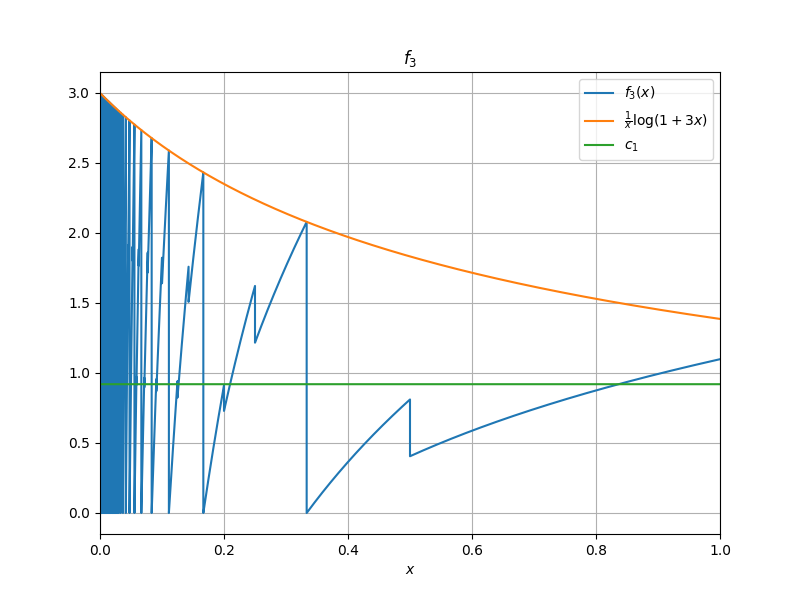
\includegraphics[width=0.5\textwidth]{discrepancy.png}
\caption{A plot of \eqref{kb}}
\label{fig:kb}
\end{figure}

From this inequality and \eqref{mod}, we
\begin{equation}\label{nup3-lower} 
\nu_p(N!/\tuple^{(3)}) \geq - O\left( \frac{N(\log\log N)^2}{p \log^2 N} \right)
\end{equation}
and thus by Mertens' theorem we obtain \eqref{deficit-targ}.  This completes the proof of \eqref{new-balance-5}.

To finish the proof of \eqref{main-lower}, it suffices by \Cref{step4-reduce} to establish the condition \eqref{sector} whenever $n_{**}, m_{**}$ obey \eqref{nstarb}.  The left-hand side of \eqref{nstarb} can be bounded by
$$ \ll \sum_{3 < p \leq t/K} \left| \nu_p\left(\frac{N!}{\tuple^{(3)}}\right) \right|\log p + \log N.$$
We claim that this expression is $O( N (\log\log N)^2 / \log N )$, which implies
$$ n_{**}, m_{**} \ll \frac{N (\log\log N)^2}{\log N}.$$
For the contribution of the primes in the range $K(1+\frac{3N/t}{A}) < p \leq t/K$ this follows readily from \eqref{anp}; the contribution of $K < p \leq K(1+\frac{3N/t}{A})$ follows readily from \eqref{tech}; and the contribution of $3 < p \leq K$ follows readily from \eqref{crude-upper}, \eqref{nup3-lower}, and Mertens' theorem.  Also, from \eqref{tinycon}, \eqref{legendre} we see for a tiny prime $p=2,3$ that
\begin{align*}
  \nu_p(N!/\tuple^{(3)}) &= \frac{N}{p-1} + O(\log N) -
O\left( \sum_{p' > t/K} \frac{N}{p'} \nu_{p}(\lceil t/p' \rceil) \right) \\
&= \frac{N}{p-1} + O(\log N)
- O\left( \sum_{p' > t/K} \frac{N}{p'} \log \log N \right)\\
&= \frac{N}{p-1} + O\left( \frac{N (\log\log N)^2}{\log N} \right)
\end{align*}
(with room to spare), and so
\begin{align*}
   \nu_2(N!/\tuple^{(3)}) - n_{**} &= N + O\left( \frac{N (\log\log N)^2}{\log N} \right)\\
   \nu_3(N!/\tuple^{(3)}) - m_{**} &= \frac{N}{2} + O\left( \frac{N (\log\log N)^2}{\log N} \right).
\end{align*}
By choice of $L$, this implies \eqref{sector} for $N$ large enough.  The proof of \eqref{main-lower} is now complete.

\section{Guy--Selfridge conjecture for \texorpdfstring{$N>10^{19}$}{N > 10\^19}}


\section{Guy--Selfridge conjecture for medium values of \texorpdfstring{$N$}{N}}



\begin{thebibliography}{10}

\bibitem{buthe}
J. B\"uthe, \emph{Estimating $\pi(x)$ and related functions under partial RH assumptions}, Math. Comp., 85(301), 2483--2498, Jan. 2016.

\bibitem{dusart}
P. Dusart, \emph{Explicit estimates of some functions over primes}, Ramanujan J. \textbf{45} (2018) 227--251.

\bibitem{guy-selfridge}
R. K. Guy, J. L. Selfridge, \emph{Factoring factorial $n$}, Amer. Math. Monthly \textbf{105} (1998) 766--767.

\bibitem{robbins}
H. Robbins, \emph{A Remark on Stirling's Formula}, Amer. Math. Monthly \textbf{62} (1955) 26--29.

\bibitem{tao}
T. Tao, \emph{Decomposing factorials into bounded factors}, preprint, 2025. \url{https://arxiv.org/abs/2503.20170}

\end{thebibliography}


\end{document}
